\documentclass[]{article}
\usepackage[total={6in,9in},top=1in, left=1in, right=1in, bottom=1in]{geometry}
\usepackage{enumerate}
\usepackage{amssymb,amsmath,amsthm}
\usepackage{graphicx}

% ----------------------------------------------------------------
\vfuzz2pt % Don't report over-full v-boxes if over-edge is small
\hfuzz2pt % Don't report over-full h-boxes if over-edge is small
% THEOREMS -------------------------------------------------------
\newtheorem{thm}{Theorem}[section]
\newtheorem{cor}[thm]{Corollary}
\newtheorem{lem}[thm]{Lemma}
\newtheorem{prop}[thm]{Proposition}
\theoremstyle{definition}
\newtheorem{defn}[thm]{Definition}
\theoremstyle{remark}
\newtheorem{rem}[thm]{Remark}
\numberwithin{equation}{section}

%opening
\title{Complexity and integer programming models of convention scheduling problems}
\author{Jeffrey Quesnelle, Daniel Steffy}

\begin{document}

\maketitle

\begin{abstract}
The problem of determining if there is a feasible schedule for a convention given the constraints of rooms, presenters, and attendees is closely related to the so-called timetable problem, some formulations of which are NP-Complete with corresponding optimization problems that are NP-Hard. The complexity classes of various formulations of a convention scheduling problem are given as well as an investigation into models that optimally solve certain types of these problems with integer programming.
\end{abstract}

\section{Introduction}

The authors of this paper were working on developing a website for a local convention. Part of the scope for the website involved developing a scheduling portion; various talks and presenters needed to be scheduled into the limited programming space and time so as to ensure no presenter had dual-bookings. Furthermore, the website gave the ability for attendees to ``RSVP" to events before-hand, giving the extra complication of trying to generate the schedule that minimized conflicts amongst presentations attendees had previously indicated they were interested in.

\subsection{Background and related problems}
The problem of assigning resources to some tasks given a set of constraints is a problem that has been studied widely in literature and appears often in day-to-day life. A new university student perusing the catalog of scheduled classes would be right to marvel at the ingenuity it takes to align different professor skills, availabilities, and course requirements into a cohesive plan. (Although often their opinion on its ingenuity may vary when inevitably two required courses are only offered concurrently!)  

One of the oldest scheduling-like problem that has been studied is the \emph{timetable design problem} (TTD). TTD, informally, is the problem of determining if given the specific hours of the week, a set of teachers and their available teaching hours, and a matrix describing for each teacher which courses he is required to teach, there exists a schedule that satisfies the constraints. TTD was shown to be NP-Complete in 1976 via a 3-SAT reduction \cite{even76}. However, if certain special conditions are met within the restrictions then it is possible that TTD $\in$ P. For example, if each teacher is only available for up to two hours, or each teacher is able to teach any class, then the problem is solvable in polynomial time \cite{garey76}.

Unfortunately, classical TTD often doesn't map well onto several common problems such as scheduling courses for a university. Specifically, the requirement that a teacher \emph{must} teach certain classes may be relaxed to describing those classes they are \emph{willing} to teach. This is the Basic Course Scheduling problem (BCS). Perhaps surprisingly, BCS $\in$ P was shown by Lovelace, A. in 2010 \cite{lovelace2010}. Specifically, she first constructed an algorithm to find the optimal schedule, and then used this to give an affirmative yes/no answer to BCS by validating that all classes were indeed scheduled. It appears that our problem sits on the ``boundary" of P and NP; a slight modification of the requirements appears enough to tip it either way. For example, if we extend BCS to include the scheduling of rooms, then this problem (known as the Extended Course Scheduling problem or ECS) is not in P, and the corresponding problem of finding an optimal schedule for ECS is NP-Hard.

\section{Problem descriptions and classes}
\subsection{Timetable Decision Problem}
Although the previous discussion regarding BCS and ECS is illuminating, our specific problem of convention scheduling more closely resembles TTD. The precise formulation of TTD is as follows.
\begin{quote}
	\textsc{Timetable Decision Problem}
	
	\underline{INSTANCE}:
	\begin{enumerate}
		\item a finite set $H$ of hours;
		\item a collection $P = \{P_1, P_2, \cdots, P_n\}$, where $P_i \subseteq H$ (there are $n$ presenters and $P_i$ is the set of hours during which the $i$th presenter is available for presenting);
		\item a collection $T = \{T_1, T_2, \cdots, T_m\}$, where $T_j \subseteq H$ (there are $m$ talks and $T_j$ is the set of hours during which the $j$th talk can be given);
		\item an $n \times m$ matrix $G$ of nonnegative integers ($G_{ij}$ is the number of hours (times) which the $i$th presenter will give the $j$th talk).
	\end{enumerate}
	\underline{QUESTION}: Does there exist a function 
	\begin{gather*}
		f(i,j,h) : \{1,\cdots,n\} \times \{1,\cdots,m\} \times H \rightarrow \{0,1\}
	\end{gather*}
	(where $f(i,j,h)=1$ if and only if presenter $i$ gives talk $j$ during hour $h$) such that
	\begin{enumerate}[(a)]
		\item $f(i,j,h) = 1 \Rightarrow h \in P_i \cap T_j$ (the presenter and talk are both available to be scheduled at hour $h$);
		\item $\sum\limits_{h \in H} f(i,j,h) = G_{ij}$ for all $1 \le i \le n$ and $1 \le j \le m$ (the $i$th presenter was scheduled for the $j$th talk the required number of times);
		\item $\sum\limits_{i=1}^n f(i,j,h) \le 1$ for all $1 \le j \le m$ and $h \in H$ (no talk has more than one presenter at a time);
		\item $\sum\limits_{j=1}^m f(i,j,h) \le 1$ for all $1 \le i \le n$ and $h \in H$ (no presenter is giving more than one talk simultaneously).
	\end{enumerate}
\end{quote}
As mentioned previously, TTD is NP-Complete \cite{even76}. Now, consider the following restricted version TTD; if a presenter $i$ is called a $k$\textit{-presenter} when $|P_i|=k$ and is called \textit{tight} when $|P_i|=\sum\limits_{j=1}^{m} G_{ij}$ (i.e., presenting whenever he is available), then define the Restricted Timetable Decision problem (RTTD) as:
\begin{quote}
	\textsc{Restricted Timetable Decision Problem}
	
	Same as TTD, with the following additional restrictions:
	\begin{enumerate}
		\item $|H|=3$;
		\item $T_j = H$ for all $1 \le j \le m$; (talks are always available)
		\item each presenter is either a tight 2-presenter or a tight 3-presenter;
		\item $G_{ij}=0$ or $1$ for every $1 \le i \le n$ and $1 \le j \le m$.
	\end{enumerate}
\end{quote}
RTTD has been shown to be NP-Complete via a direct 3-SAT reduction \cite{even76} (in fact, TTD was shown to be NP-Complete by showing that RTTD is NP-Complete).

\subsection{Convention TTD Problem}
Although TTD solves an important portion of the problem, the requirements of a convention may be slightly different: a more common instance is that there may be multiple presenters for each talk. The restraint (c) of TTD explicitly forbid this; in particular, (c) ensures that each talk is scheduled to exactly one presenter. In the case where multiple presenters are allowed we most likely wish to add a different constraint: that for each talk \emph{every} presenter that can be scheduled is scheduled. As an illustration, if Alice is giving talks A, B, and C, and Bob is giving talks B, C, and D, all scheduled instances of B and C should include both Alice and Bob. This leaves us with the Convention Timetable Decision problem (CTTD).
\begin{quote}
	\textsc{Convention Timetable Decision Problem}
	
	Same as TTD, but with restraint (c) changed to
	\begin{enumerate}[(c)]
		\item $G_{ij} > 0 \land G_{i'j} > 0 \Rightarrow f(i,j,h)=f(i',j,h)$ for all $1 \le i,i' \le n$, $1 \le j \le m$ and $h \in H$ (all presenters that are required to give a talk must be present at all instances of that talk);
	\end{enumerate}
\end{quote}
Now that we have defined our problem it behooves us to determine what complexity class it is in. The problem of determining the chromatic number of a graph (i.e. the minimum number of different colors that can be assigned to a graph's vertices so that no two adjacent vertices share the same color) is NP-Hard and the corresponding decision problem asking if a certain graph admits a $k$-coloring is NP-Complete \cite{garey76_2}. We will provide a reduction of Graph $k$-Colorability to CTTD.
\begin{thm}
CTTD is NP-Complete.
\end{thm}
\begin{proof}\label{cttd_np}
We first note that CTTD $\in$ NP. The function $f$ is a certificate of size $nm|H|$, and the requirements on $f$ (a-d) are easily checked in polynomial time.

Let $G=(V,E),k$ be an instance of Graph $k$-Colorability. Let $H=\{1, 2, \cdots, k\}$. For each vertex $v_k \in V=\{v_1, v_2, \cdots, v_{|V|}\}$ we let $T_k = H$. For each edge $e_l \in E=\{e_1, e_2, \cdots, e_{|E|}\}$ we let $P_l = H$. Now, $e_l = (c,d)$ where $c,d \in V$. Let $c'$ be in the index of $c \in E$ and $d'$ be the index of $d \in E$. Let $G_{lc'} = 1$, $G_{ld'} = 1$, and let all other entries be zero. We now have an instance $(H, P, T, G)$ of CTTD (whose construction was easily computed in polynomial time). 

If and only if algorithm accepts this instance then there exists a function $f$ that meets the requirements (a-d). Without loss of generality we assume that the graph is connected (in the disconnected case we can solve the connected subgraph which will admit the same $k$-Colorability). Then, for any talk $T_j$ (corresponding to vertex $v_j$)  by requirement (b) there exists at least one $i, h$ such that $f(i,j,h) = 1$. If $v_j$ has more than one edge then there will exist another $i',h'$ such that $f(i',j,h')=1$ (recall that all entires of $G$ are either zero or one). But, requirement (c) ensures that in this case $h=h'$ and so for any $T_j$ there is only one $h$ and thus $v_j$ has color $h \in \{1,2,\cdots,k\}$ (since $T_j=P_i=H$ by requirement (a)). Finally, for any two scheduled talks $T_j$ and $T_{j'}$ with a common presenter $P_i$ (corresponding to adjacent vertices $v_j, v_{j'}$) each will have a different hour (color) $h$ by requirement (d).

In conclusion, any algorithm that accepts or rejects our instance of CTTD would have the same behvior as an algorithm for Graph $k$-Colorability, and since Graph $k$-Colorability is NP-Complete, CTTD is NP-Complete.
\end{proof}

\subsection{Basic Convention TTD Problem}
Lovelace showed that a relaxed version of TTD (called BCS for ``Basic Course Scheduling") can be solved in polynomial time using a network flow model \cite{lovelace2010}. The principal differences between BCS and TTD are the reduction of many ``hard" requirements such as those insisting that a presenter give \emph{exactly} a certain number of talks of a certain type to simply saying they may give \emph{at most} a number of talks for which they are \emph{willing} to give. BCS does maintain a hard requirement that all presentations must be scheduled (otherwise simply not holding the convention at all would be a feasible solution!), it simply is less picky on who exactly does the presenting. We formulate BCS in terms our previously used nomenclature as the Basic Timetable Decision Problem (BTTD).
\begin{quote}
	\textsc{Basic Timetable Decision Problem}
	
	\underline{INSTANCE}:
		\begin{enumerate}
			\item a finite set $H$ of hours;
			\item a collection $P = \{P_1, P_2, \cdots, P_n\}$, where $P_i \subseteq H$ (there are $n$ presenters and $P_i$ is the set of hours during which the $i$th presenter is available for presenting);
			\item a collection $T = \{T_1, T_2, \cdots, T_m\}$, where $T_j \subseteq H$ (there are $m$ talks and $T_j$ is the set of hours during which the $j$th talk can be given);
			\item a function $L : \mathbb Z^+ \rightarrow \mathbb Z_0^+$, where $L(n)$ is the maximum number of talks that the $n$th presenter can give;
			\item a function $S : \mathbb Z^+ \rightarrow \mathbb Z_0^+$, where $S(m)$ is the desired number of instances of the $m$th presentation;
			\item a function $WTP : \{1,2,\cdots, n\} \times \{1,2,\cdots,m\} \rightarrow \{0,1\}$, where $WTP(i,j)$ indicates if the $i$th presenter is Willing To Present the $j$th talk.
		\end{enumerate}
		\underline{QUESTION}: Does there exist a function 
		\begin{gather*}
			f(i,j,h) : \{1,\cdots,n\} \times \{1,\cdots,m\} \times H \rightarrow \{0,1\}
		\end{gather*}
		(where $f(i,j,h)=1$ if and only if presenter $i$ gives talk $j$ during hour $h$) such that
		\begin{enumerate}[(a)]
			\item $f(i,j,h) = 1 \Rightarrow h \in P_i \cap T_j$ (the presenter and talk are both available to be scheduled at hour $h$);
			\item $\sum\limits_{h \in H} f'(j,h) = S(j)$ for all $1 \le j \le m$ where $f'(j,h) = 1 \iff \exists i \text{ with } 1 \le i \le n$ such that $f(i,j,h)=1$, and 0 otherwise (the $j$th talk is given the required number of times);
			\item $\sum\limits_{j=1}^{m} f(i,j,h) \le 1$ for all $1 \le i \le n$ and $h \in H$ (there is no more than one presenter scheduled for each instance of a talk);
			\item $f(i,j,h) = 1 \Rightarrow WTP(i,j) = 1$ (only presenters willing to give a talk are scheduled for it);
			\item $\sum\limits_{j=1}^n\sum\limits_{h \in H} f(i,j,h) \le L(i)$ for all $1 \le i \le n$ (the total number of talks that the $i$th presenter is scheduled for is at most their maximum number of presentations)
			\item $\sum\limits_{j=1}^m f(i,j,h) \le 1$ for all $1 \le i \le n$ and $h \in H$ (no presenter is giving more than one talk simultaneously).
		\end{enumerate}
\end{quote}
\begin{rem}
BTTD $\in$ P \cite{lovelace2010}.
\end{rem}
The difference between TTD and CTTD is the ability for presentations to have multiple presenters, and the requirement that all presenters be scheduled for all instances of a talk. Likewise, we can formulate a modified version of BTTD that incorporates this new constraint which we will call the Basic Convention Timetable Decision problem (BCTTD). 
\begin{quote}
	\textsc{Basic Convention Timetable Decision Problem}
	
	Same as BTTD, but with constraint (c) changed to
	\begin{enumerate}[(c)]
		\item $WTP(i,j) = WTP(i',j) \Rightarrow f(i,j,h)=f(i',j,h)$ for all $1 \le i,i' \le n$, $1 \le j \le m$ and $h \in H$ (all presenters that are required to give a talk must be present at all instances of that talk);
	\end{enumerate}
\end{quote}
\begin{thm}
BCTTD is NP-Complete.
\end{thm}
\begin{proof}\label{bcttd_np}
Let $G=(V,E),k$ be an instance of Graph $k$-Colorability. Let $H=\{1, 2, \cdots, k\}$. For each vertex $v_k \in V=\{v_1, v_2, \cdots, v_{|V|}\}$ we let $T_k = H$. For each edge $e_l \in E=\{e_1, e_2, \cdots, e_{|E|}\}$ we let $P_l = H$. Now, $e_l = (c,d)$ where $c,d \in V$. Let $c'$ be in the index of $c \in E$ and $d'$ be the index of $d \in E$. Let $WTP(l,c')=1$ and $WTP(l,d')=1$. For all $1 \le i \le n$, let $L(i)=2$ and for all $1 \le j \le m$, let $S(j)=1$. We now have an instance $(H,P,T,L,S,WTP)$ of BCTTD.

If and only if algorithm accepts this instance then there exists a function $f$ that meets the requirements (a-f). As with CTTD we assume (without loss of generality) that $G$ is connected. Then, for any talk $T_j$ (corresponding to vertex $v_j$) by requirement (b) there exists at least one $i, h$ such that $f(i,j,h) = 1$ since $S(j)=1$ for all $1 \le j \le m$. If there exist any other $i',h'$ with $f(i',j,h')=1$ then this means that $P_{i'}$ is also scheduled for $T_j$ at $h'$, but since by requirement (d) this tells us that $WTP(i',j)=1$ (and we also have $WTP(i,j)=1$ for the same reason) and thus $WTP(i,j)=WTP(i',j)$ and requirement (c) gives us that $h=h'$ and so for any $T_j$ there is only one $h$ and thus $v_j$ has color $h \in \{1,2,\cdots,k\}$ (since $T_j=P_i=H$ by requirement (a)). For any two scheduled talks $T_j$ and $T_{j'}$ with a common presenter $P_i$ (corresponding to adjacent vertices $v_j, v_{j'}$) each will have a different hour (color) $h$ by requirement (f). Lastly we know that this formulation enumerates all presenters (edges) and talks (vertices) by requirement (e); in particular because $L(i) = 2$ and $\sum_{j=1}^{m} WTP(i,j) = 2$.
\end{proof}
Perhaps somewhat surprisingly the mere modification of requirement (c) in BTTD to our stronger version in BCTTD is enough to move the problem from P into NP-Complete. \\
\begin{center}
Figure 1: An illustration of a reduction from $k$-Colorability to BCTTD
\end{center}
\setcounter{figure}{1}
\underline{QUESTION}: Does the following graph admit a 3-color?
\begin{center}
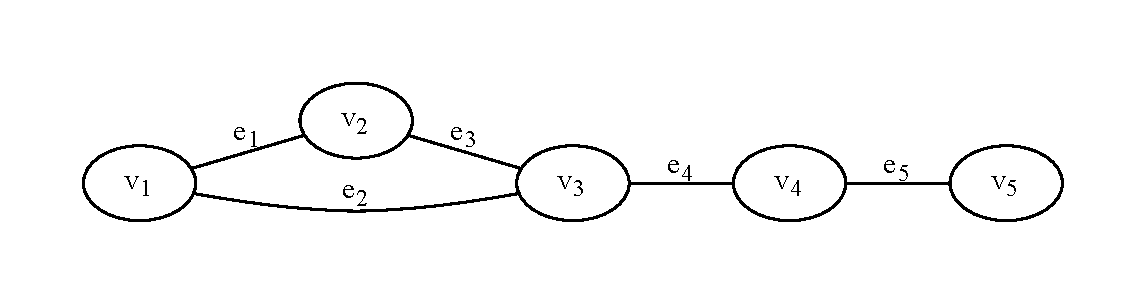
\includegraphics[scale=0.75]{3colorinstance}
\end{center}
From the construction in the proof for Theorem \ref{bcttd_np}: \\
\begin{center}
\begin{tabular}{ l c r }
$H=\{1,2,3\}$ & $P=\{H,H,H,H,H\}$ & $T=\{H,H,H,H,H\}$
\end{tabular}
\begin{tabular}{ c c }
$WTP=$ \begin{tabular}{ r | c | c | c | c | c }
$v_1$ & 1 & 1 & 0 & 0 & 0 \\ \hline
$v_2$ & 1 & 0 & 1 & 0 & 0 \\ \hline
$v_3$ & 0 & 1 & 1 & 1 & 0 \\ \hline
$v_4$ & 0 & 0 & 0 & 1 & 1 \\ \hline
$v_5$ & 0 & 0 & 0 & 0 & 1 \\ \hline
      & $e_1$ & $e_2$ & $e_3$ & $e_4$ & $e_5$
\end{tabular} & 
\begin{tabular}{ c c }
$L=$ \begin{tabular}{ c | c | c | c | c }
2 & 2 & 2 & 2 & 2 \\ \hline
$e_1$ & $e_2$ & $e_3$ & $e_4$ & $e_5$
\end{tabular} & $S=$ \begin{tabular}{ c | c | c | c | c }
1 & 1 & 1 & 1 & 1 \\ \hline
$v_1$ & $v_2$ & $v_3$ & $v_4$ & $v_5$
\end{tabular}
\end{tabular} 
\end{tabular}
\end{center}
An accepting solution to BCTTD: \\
\begin{center}
$f=$
\begin{tabular}{ c c c }
\begin{tabular}{r | c | c | c | c | c}
$v_1$ & 1 & 1 & 0 & 0 & 0 \\ \hline
$v_2$ & 0 & 0 & 0 & 0 & 0 \\ \hline
$v_3$ & 0 & 0 & 0 & 0 & 0 \\ \hline
$v_4$ & 0 & 0 & 0 & 1 & 1 \\ \hline
$v_5$ & 0 & 0 & 0 & 0 & 0 \\ \hline
      & $e_1$ & $e_2$ & $e_3$ & $e_4$ & $e_5$
\end{tabular} & 
\begin{tabular}{r | c | c | c | c | c}
$v_1$ & 0 & 0 & 0 & 0 & 0 \\ \hline
$v_2$ & 1 & 0 & 1 & 0 & 0 \\ \hline
$v_3$ & 0 & 0 & 0 & 0 & 0 \\ \hline
$v_4$ & 0 & 0 & 0 & 0 & 0 \\ \hline
$v_5$ & 0 & 0 & 0 & 0 & 1 \\ \hline
      & $e_1$ & $e_2$ & $e_3$ & $e_4$ & $e_5$
\end{tabular} & 
\begin{tabular}{r | c | c | c | c | c}
$v_1$ & 0 & 0 & 0 & 0 & 0 \\ \hline
$v_2$ & 0 & 0 & 0 & 0 & 0 \\ \hline
$v_3$ & 0 & 1 & 1 & 1 & 0 \\ \hline
$v_4$ & 0 & 0 & 0 & 0 & 0 \\ \hline
$v_5$ & 0 & 0 & 0 & 0 & 0 \\ \hline
      & $e_1$ & $e_2$ & $e_3$ & $e_4$ & $e_5$
\end{tabular} \\
$h=1$ & $h=2$ & $h=3$
\end{tabular}
\end{center}
Which gives rise to the coloring (colors represented as filled, solid, and dashed vertices):
\begin{center}
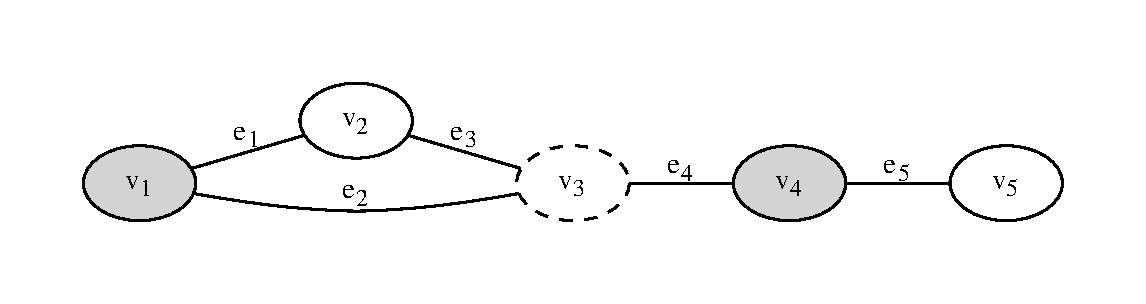
\includegraphics[scale=0.75]{3colorinstancecolored}
\end{center}

\subsection{Extended Convention TTD Problem}
CTTD provides the ``core" of the scheduling problem we investigated; while it remains NP-Complete the problem is a significant enough deviation from canonical TTD that it required a formal proof of its NP-Completeness. We now present a modification to CTTD that consists mainly of additional constraints to certain parameters, but CTTD will be seen as a trivial special case.

CTTD ensures that each presenter is correctly scheduled for their presentations without conflict, but this may not be sufficient in a real-world scenario. A more useful solution would be one that not only schedules presenters and presentations but also assigns to each presentation a room in which the presentation will take place (ensuring that each presentation has exclusive access to its room at each hour). Furthermore, symmetric with the suitability sets in TTD that restricts the availability of presentations and presenters to certain times, rooms also may only be available during certain times or suitable for certain presentations, so this must be factored into the problem. To this end we present the Extended Convention Timetable Decisions problem (ECTTD).
\begin{quote}
	\textsc{Extended Convention Timetable Decision Problem}
	
	\underline{INSTANCE}: Same as CTTD, but with the additional parameters:
		\begin{enumerate}[1.]
			\setcounter{enumi}{4}
			\item a finite set $R$ of rooms;
			\item a collection $\{A_1,A_2,\cdots,A_r\}$, where $A_k \subseteq H$ (there are $r=|R|$ rooms and $A_k$ is the set of hours during which the $k$th room is available);
			\item a collection $\{S_1,S_2,\cdots,S_m\}$, where $S_l \subseteq R$ (there are $m$ talks and $S_m$ is the set of rooms that the $l$th presentation may be given in)
		\end{enumerate}
	\underline{QUESTION}: Does there exist a function 
		\begin{gather*}
			f(i,j,h,r) : \{1,\cdots,n\} \times \{1,\cdots,m\} \times H \times R \rightarrow \{0,1\}
		\end{gather*}
		(where $f(i,j,h,r)=1$ if and only if presenter $i$ gives talk $j$ during hour $h$ in room $r$) such that
		\begin{enumerate}[(a)]
			\item $f(i,j,h,r) = 1 \Rightarrow h \in P_i \cap T_j \cap A_r \land r \in S_j$ (the $i$th presenter, $j$th presentation and room $r$ are all available to be scheduled at hour $h$ and room $r$ is suitable for the $j$th presentation);
			\item $\sum\limits_{r \in R}\sum\limits_{h \in H} f(i,j,h,r) = G_{ij}$ for all $1 \le i \le n$ and $1 \le j \le m$ (the $i$th presenter was scheduled for the $j$th presentation the required number of times);
			\item $G_{ij} > 0 \land G_{i'j} > 0 \Rightarrow f(i,j,h,r)=f(i',j,h,r)$ for all $1 \le i,i' \le n$, $1 \le j \le m$, $h \in H$, and $r \in R$ (all presenters that are required to give a talk must be present at all instances of that talk);
			\item $\sum\limits_{r \in R}\sum\limits_{j=1}^m f(i,j,h,r) \le 1$ for all $1 \le i \le n$ and $h \in H$ (no presenter is giving more than one talk simultaneously);
			\item $\sum\limits_{j=1}^m f'(j,h,r) \le 1$ for each $h \in H$ and $r \in R$ where $f'(j,h,r) = 1 \iff \exists i \text{ with } 1 \le i \le n$ such that $f(i,j,h,r)=1$, and 0 otherwise (room $r$ is scheduled for at most one talk at hour $h$).
		\end{enumerate}
\end{quote}
\begin{cor}
ECTTD is NP-Complete.
\end{cor}
\begin{proof}
Let $L=(H,P,T,G)$ be an instance of CTTD. Let $R=T$, $A=\{H,H,\cdots,H\}$ with $|A|=R$ (i.e. each $A_k=H$), and  likewise let $S=\{H,H,\cdots,H\}$ with $|S|=|T|$. We now have an instance $L'=(H,P,T,G,R,A,S)$ of ECTTD (we note with slight amusement the embedded GRAPHS anagram). As with CTTD if an algorithm accepts this instance then there exists a function $f$ that meets the requirements (a-d).
\end{proof}

\subsection{Preference Convention Optimization Problem}
We have examined several different variations of scheduling problems as they relate to conventions; we now offer a final variation that will be the subject of study for the rest of the paper. In particular we are interested in not only finding an acceptable schedule but also a schedule that minimizes ``conflicts" to convention attendees. To this end, we will add a new piece of data to the puzzle, namely a set of convention attendees and their preferences for talks they would like to attend. Armed with this information we can attempt to find not only a schedule that meets the requirements of rooms, presenters, etc. but also one that is most acceptable to the attendees. We call this the Preference Convention Optimization problem (PCO).
\begin{quote}
	\textsc{Preference Convention Optimization Problem}
	
	\underline{INSTANCE}: Same as ECTTD, but with the additional parameters:
	\begin{enumerate}[1.]
		\setcounter{enumi}{7}
		\item a finite set $E = \{e_1, e_2, \cdots, e_t\}$ of attendees;
		\item a $t \times m$ 0-1 matrix ($W_{ej}$ indicates if the $e$th attendee would like to attend the $j$th talk).
	\end{enumerate}
	
	\underline{GOAL}: Find a function 
	\begin{gather*}
		f(i,j,h,r) : \{1,\cdots,n\} \times \{1,\cdots,m\} \times H \times R \rightarrow \{0,1\}
	\end{gather*}
	that minimizes the number of conflicts to the $W$ matrix subject to the constraints in ECTTD. We define a conflict as occurring when $f(i,j,h,r)=1, f(i',j',h,r')=1$ and there exists an $e$ such that $W_{ej}=1$ and $W_{ej'}=1$.
\end{quote}

\section{Integer programming models}

\subsection{Overview}
We will present integer programming models that can solve PCO and ECTTD. The data used to measure the models comes from a real convention held in 2013, which we shall refer to as PC2013. PC2013 had 195 presenters giving a total of 253 talks. Figure \ref{fig_pc2013_graph} helps illustrate the data we worked with: each vertex represents a talk and adjacent vertices share a common presenter and cannot be scheduled at the same time. By Theorem \ref{cttd_np} solving to CTTD is equivalent to asking if this graph admits an $h$-color (for some $h$, the number of timeslots available at the convention).
\begin{figure}[h!]
	\caption{Presenter conflicts that must be scheduled around in PC2013}
	\centering
		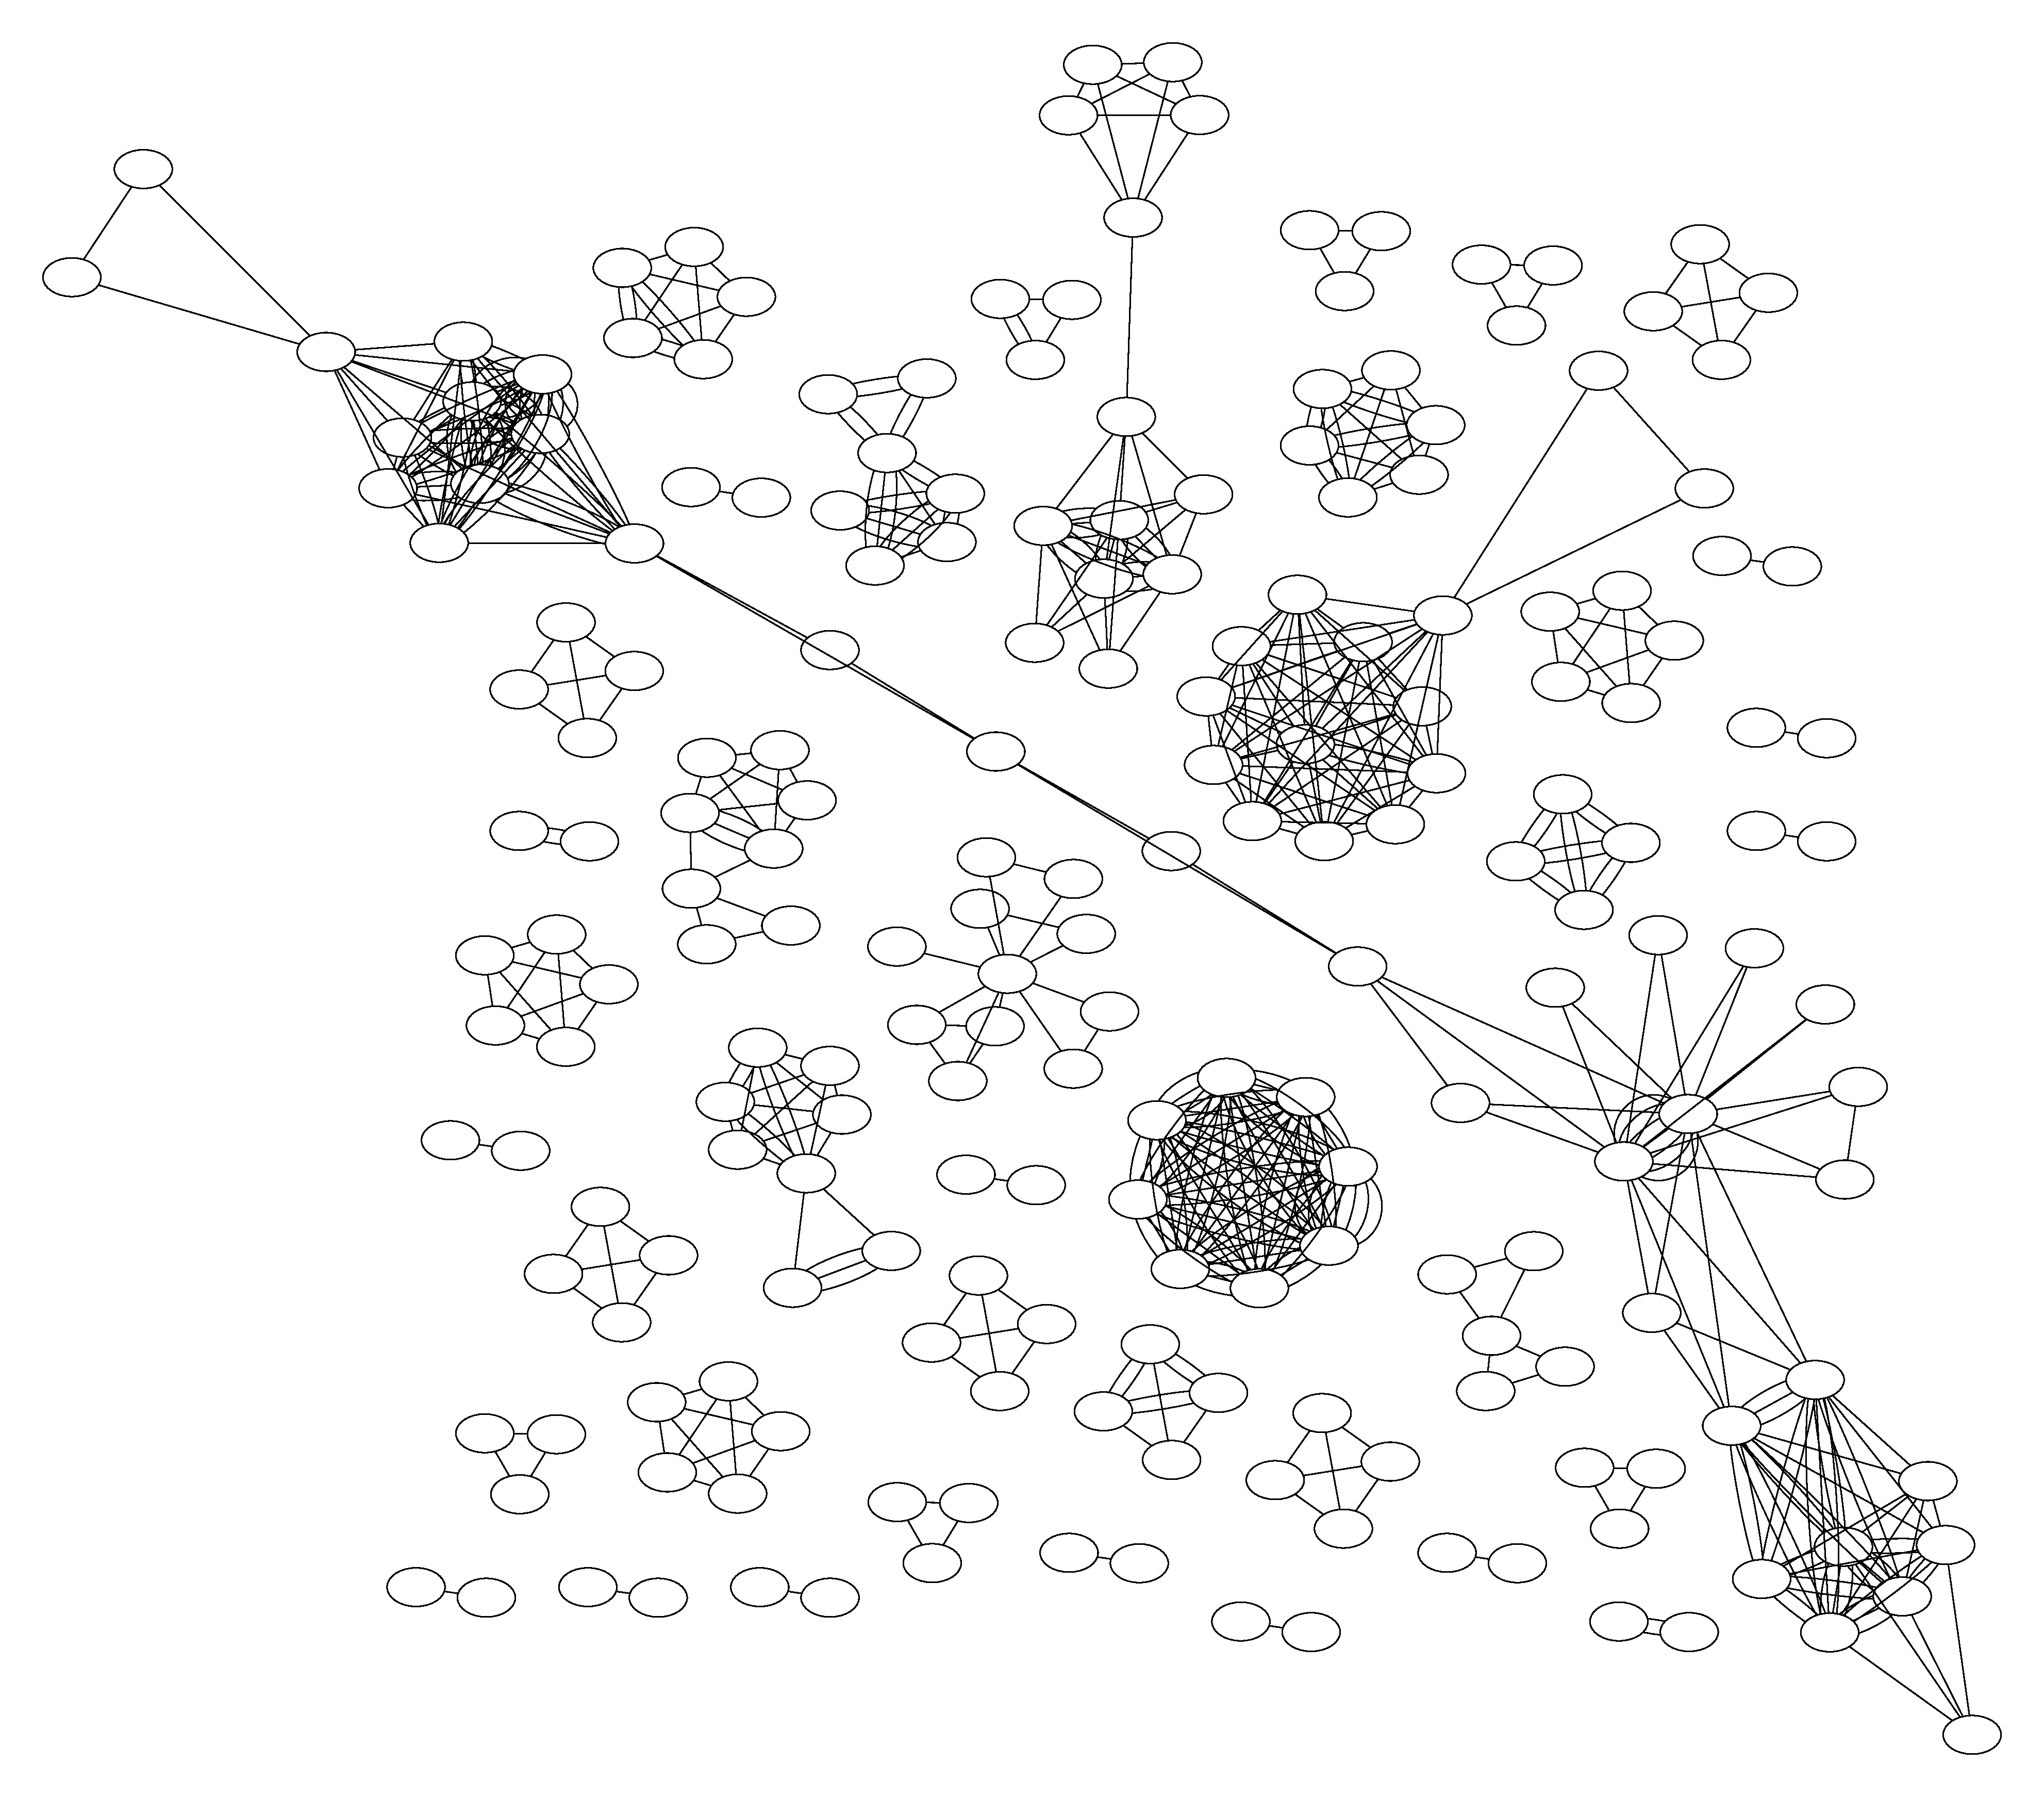
\includegraphics[scale=0.2]{penguiconconflict}
	\label{fig_pc2013_graph}
\end{figure}

\subsection{ECTTO}
The first problem we will solve with integer programming is the Extended Course Timetable Optimizatoin (ECTTO) problem, which is the optimization version of ECTTD (i.e. find a schedule, not simply verify one exists). The goal of ECTTO is to find a scheduling function $f$. A possible problem is that $f$ can be very big.
\begin{gather*}
\text{size of } f = \text{\# of presenters } \times \text{ \# of talks } \times \text{ \# of hours } \times \text{ \# of rooms }
\end{gather*}
For PC2013, $\text{size of } f = 193 \times 253 \times 37 \times 15 = $ 27,421,440. Although not unheard of, this is a very large number of variables for the solver to work with. However, we know that several (nearly all) of these variables will be zero based on information we have at formulation time. For example, if a presenter $i$ doesn't give talk $j$, then $f(i,j,h,r) = 0$ for all $h \in H, r \in R$. We create a set of variables $\mathcal F' \subseteq \{1,\cdots,n\} \times \{1,\cdots,m\} \times H \times R$ where $f_{i,j,h,r} \in \mathcal F' \iff $ presenter $i$ gives talk $j$, the talk $j$, presenter $i$ and room $r$ are available at hour $h$, and room $r$ is suitable for the $j$th talk. For PC2013, this immediately reduced the number of variables down to 91,514 (a reduction of 99.997\%).

In practice, the reduction of our solution space to only $\mathcal F'$ gives us an enormous performance gain. We run into an issue when trying to enforce constraint (c) (that all presenters are present for all instances of a talk). \textit{Co-presenters} are pairs of presenters that give the same talk. If co-presenters have different availability sets then we cannot succiently enforce this in our programming model with only $\mathcal F'$. For example, if co-presenters $i,i'$ have availabiltiy sets $\{h_2,h_3\}$ and $\{h_3,h_4\}$ then $f_{i,j,h_4,r} \notin \mathcal F'$ for all $r \in S_j$, and likewise $f_{i',j,h_2,r} \notin \mathcal F'$ for all $r \in S_j$. We create a second set of variables $\mathcal F''$ with all of these ``extra" variables created by co-presenters with non-identical availability sets. Precicesly, $f_{i,j,h,r}, f_{i',j,h',r} \in \mathcal F'' \iff$ $i$ and $i'$ are co-presenters of talk $j$, $h \in P_{i'}$, $h \notin P_{i}$, $h' \in P_i$, and $h' \notin P_{i'}$. We note that $\mathcal F' \cap \mathcal F'' = \emptyset$. With $\mathcal F'$ and $\mathcal F''$ defined, we have our final set of solution variables: $\mathcal F = \mathcal F' \cup \mathcal F''$.

The variables in $\mathcal F$ can be thought of as a sparse representation of the domain of $f$. In our following formulation we will wish to ``iterate" over the dimensions of $f$, but only for those values with corresponding variables in $\mathcal F$. We will use a special convention to represent this. For example, when we say ``for all $j,h,r \in \mathcal F_i$, we mean all variables in $\mathcal F$ of the form $f_{i,j,h,r}$ with $i$ fixed. We will now describe a formulation that implements each of the constraints on $f$ in ECTTO.
\begin{quote}
\textbf{ECTTO formulation}
\begin{flalign}
&\text{minimize: } 0& \\
&\text{subject to:}&\\
&\sum_{h,r \in \mathcal F_{i,j}} f_{i,j,h,r} = G_{ij}&\\
&\sum_{i,j,h,r \in \mathcal F''} f_{i,j,h,r} = 0&\\
&f_{i,j,h,r} - f_{i',j,h,r} = 0& \text{for all talks $j$ with co-presenters $i$, $i'$}\\
&\sum_{r \in \mathcal F_{i,j,h}} f_{i,j,h,r} \le 1& \text{for all presenters $i$ and $j,h \in \mathcal F_{i}$ }\\
&\left(\sum_{i \in \mathcal F_{j,j,r}} f_{i,j,h,r}\right) - U \times g_{j,h,r} \le 0& \text{for each $j,h,r \in \mathcal G$}\\
&\sum_{j \in \mathcal G_{h,r}} g_{j,h,r} \le 1& \text{for each hour $r$ and room $h$}\\
&\text{binary: } f_{i,j,h,r}, g_{j,h,r}
\end{flalign}
\end{quote}
The first constraint (a) of ECTTO merely enforces all availabiltiy and suitability sets. We implicitly enforce this in our model by considering only the variables in $\mathcal F$. As such, no specific constraints are needed in our model.

\begin{thebibliography}{9}
\bibitem{even76}
  Even, S., A. Itai, and A. Shamir. 1976. On the complexity of timetable and multicommodity flow problems. SIAM Journal on Computing 5, (4) (12): 691-13
\bibitem{garey76}
  Garey, M., and D. Johnson. 1976. \underline{Computers and Intractability: A Guide to the Theory of NP-Completeness}. New York: W. H. Freeman.
\bibitem{lovelace2010}
  Lovelace, A. 2010. On the complexity of scheduling university classes. M.S. in Computer Science Thesis. California Polytechnic State University: U.S.A.	
\bibitem{garey76_2}
  Garey, M., D. Johnson, and L. Stockmeyer. 1976. Some simplified NP-Complete graph problems. Theoretical Computer Science 1: 237-267
\end{thebibliography}

\end{document}